En esta sección se explica el desarrollo del proyecto y el análisis de la implementación. Para facilitar la comprensión se ha separado en diferentes etapas.

\subsection{Usuarios}
Para el desarrollo de la gestión de usuarios se han usado diferentes librerías auth y contrib principalmente. Estas librerías permiten guardar los datos de usuarios más básicos y herramientas para validarlos.

Para la gestión de usuarios se ha añadido el modulo llamado account que mediante diferentes endpoints permite la ejecución de views que realizan gran parte del trabajo.
\subsubsection{SignUp}
La creación de las cuentas de usuario se tienen que realizar mediante un template(i.e. no se h habilitado ningún endpoint de la API). El objetivo es que usuarios puedan crear aplicaciones que usen nuestra API. El formulario que podemos ver en la figura ~\ref{fig:sign_up_test}

\begin{figure}[ht!]
\center
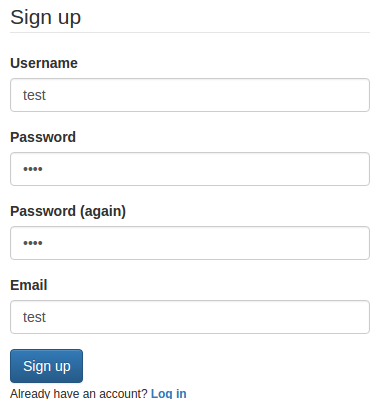
\includegraphics[scale=0.7]{screenshots/sign_up_test.PNG}
\caption{Registro de un usuario}
\label{fig:sign_up_test}
\end{figure}

Como podemos ver en el formulario se pide la confirmación del password. Para ellos se ha añadido validación de campos. En la figura ~\ref{fig:sign_up_error} podemos ver el formulario. 
\begin{figure}[ht!]
\center
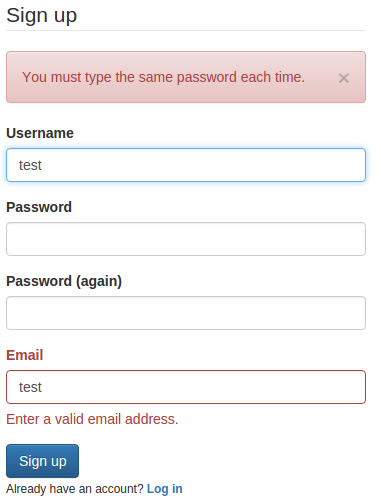
\includegraphics[scale=0.7]{screenshots/sign_up_error.PNG}
\caption{Mensajes de error en el registro}
\label{fig:sign_up_error}
\end{figure}

La validación de campos se hace de la siguiente forma.
\newpage
Aquí podemos ver el código del templete:
\begin{lstlisting}[language=HTML]
<form id="signup_form" method="post" action="" 
autocapitalize="off" 
enctype="multipart form-data">
	<legend></legend>
	
	{{ form|bootstrap }}
	
	 <input type="hidden" name="{{ redirect_field_name }}"
	 value="{{ redirect_field_value }}" />
	
	<button type="submit" class="btn btn-primary">
		
	</button>
</form>
\end{lstlisting}


Aprovecharemos la oportunidad para explicar como funciona el sistema de templates de django, el código que se encuentra entre los tags \{\% \textit{codigo} \%\} es código python que modifica el comportamiento de forma dinámica. Por otro lado el comando csrf\_token añade seguridad  contra los ataque Cross Site Request Forgery a los formularios.

Viendo el código nos preguntamos como se añaden los campos al formulario, esto se hace de la siguiente forma, el tag \{\{form\}\} lo que hace es inyectar los campos que se encuentran en la clase especificada en la vista que ``action'' dispara, para ello la vista tiene que disponer del atributo from\_class y se tiene asignar la clase que hereda de django.forms.Form donde están especificados los atributos. Para más clarificación  se adjunta el código del caso concreto que estamos viendo.

\begin{lstlisting}[language=python]
class SignupForm(forms.Form):

    username = forms.CharField(
        label=_("Username"),
        max_length=30,
        widget=forms.TextInput(),
        required=True
    )
    password = forms.CharField(
        label=_("Password"),
        widget=forms.PasswordInput(render_value=False)
    )
    password_confirm = forms.CharField(
        label=_("Password (again)"),
        widget=forms.PasswordInput(render_value=False)
    )
    email = forms.EmailField(
        label=_("Email"),
        widget=forms.TextInput(), required=True)

    code = forms.CharField(
        max_length=64,
        required=False,
        widget=forms.HiddenInput()
    )
    
class SignupView(FormView):
	...
    form_class = SignupForm
    ...
\end{lstlisting}

El registro de un usuario inicia automáticamente la validación del correo electrónico y así también la validación de la cuenta.
\paragraph{Confirmación}.\\
Para la verificación de la cuenta se ha añadido confirmación vía correo electrónico. 
Para ello se dispone de dos clases que permiten almacenar los correos electrónicos de los usuarios y se estos han estado verificados o no y otra que contiene la llave que se tiene que usar para verificar la cuenta.

El proceso de verificación empieza cuando el usuario se crea una cuenta de usuario, entonces se envía un correo  al usuario con la url que contiene la llave de validación.


{domain}/accounts/confirm\_email/{key}/

Esta URL ejecuta la vista encargada de validar la cuenta, y nos muestra una interfaz desde la que confirmar el correo (~\ref{fig:confirm_email}).
\begin{figure}[ht!]
\center
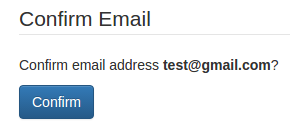
\includegraphics[scale=1.0]{screenshots/confirm_email.PNG}
\caption{Pantalla de confirmación del correo electrónico}
\label{fig:confirm_email}
\end{figure}

Al confirmar nos redirige a la pantalla de log in que podemos ver en la figura ~\ref{fig:login}.

\subsubsection{LogIn}
Para entrar lo podremos hacer con el botón que encontramos arriba a la derecha, que hará que se renderice el template de log in (figura \ref{fig:login}).
\begin{figure}[ht!]
\center
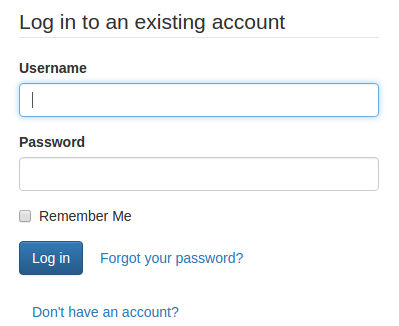
\includegraphics[scale=1.0]{screenshots/login.PNG}
\caption{Interface para entrar}
\label{fig:login}
\end{figure}

Una vez se introducen las credenciales correctamente y se pulsa sobre el botón Log in esto ejecuta la vista asociada. Esta vista ejecuta la función login de la librería django.contrib.auth, que guarda el id del usuario usando la librería sesión de django, que gestiona las cookies. Con la función sesión.set\_expiry(0) haremos que la sesión se mantenga abierta hasta que el navegador limpie las cookies.

% DELETE AND UPDATE ACCOUNT AND RESTORE PASSWORD

\subsection{Gestión de aplicaciones}
Para facilitar la autenticación de los usuarios mediante oatuh 2 se ha utilizado la librería oatuh2 toolkit, esta librería nos proporciona todas las clases necesarias para poder usar este protocolo. Las clases que esta librería nos crea en el sistema son las siguientes.
\begin{description}
\item[Applications]: En esta clase se almacenaran las aplicaciones dadas de alta por los usuarios. Estas aplicaciones podrán conseguir tokens de otros usuarios mediante el uso del protocolo establecido.
\item[AccesTokens]: En esta clase se almacenan los acces token que son validos en este momento y ligados al usuario que pertenecen. Cada acces token tiene un tiempo de vida que también se almacena en esta clase.
\item[RefreshToken]: Cada acces token tiene asignado un refresh token para poder refrescar un token al que el tiempo de vida se le haya acabado.
\end{description}

Una vez accedamos a la gestión de aplicaciones encontramos la interface desde la que podremos crear aplicaciones como podemos ver en la figura ~\ref{fig:create_aplication}.
\begin{figure}[ht!]
\center
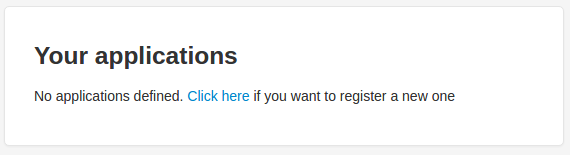
\includegraphics[scale=1.0]{screenshots/create_aplication.PNG}
\caption{Interfaces para ver las aplicaciones}
\label{fig:create_aplication}
\end{figure}

Al pulsar sobre el link que nos indica, nos dirigirá a un formulario donde podremos crear la aplicación, el formulario lo podemos ver en la figura ~\ref{fig:create_aplication2}
\begin{figure}[ht!]
\center
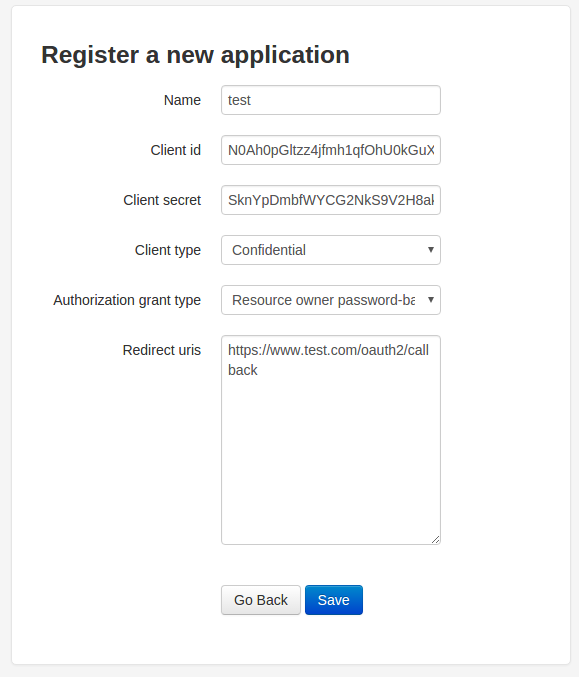
\includegraphics[scale=1.0]{screenshots/create_aplication2.PNG}
\caption{Formulario para la creación de aplicaciones}
\label{fig:create_aplication2}
\end{figure}

Los campos client id y client secret se nos llenaran automáticamente, en este caso client type y authorization type se dejan escoger por cuestiones practicas a la hora de desarrollar pero también se fijarían automáticamente en una version de producción. En este caso solo se ha testeado la autorización con gran type Resource owner password-based, en la que la aplicación gestiona las credenciales de los usuarios que ha de autenticar contra nuestra aplicación. No se entrara en detalle de como se implementa ya que lo gestiona el framework oauth2 toolkit y no tiene más complejidad que dar de alta la aplicación en nuestra base de datos.

\subsection{Endpoints}
Los endpoints son los que dan las funcionalidades de la API. Se explicaran de forma pormenorizada pero en 2 grupos ya que si bien nuestra API da servicio para gestionar muchos recursos la implementación conceputalmente es muy parecida entre ellos como ya se deducía en la especificación y diseño. Estos 2 grupos son los endpoints que realizan las operaciones CRUD y los endpoints con funcionalidades más especificas que funcionan de forma asíncrona mediante celery. También se explicara el funcionamiento de django rest framework (DRF)

\subsubsection{CRUD}
Las operaciones crud se realizan mediante diferentes endpoints siguiendo el estilo rest-ful. Para definir las urls por donde se podrá aceder a estas operaciones se definen mediante el uso de la clase router a continuación se adjunta un ejemplo:
\begin{lstlisting}[language=python]
router.register(
    r'person',
    views_genetree.PersonViewSet,
    base_name='person')
\end{lstlisting}

Este codigo hara que todas las request a la url 
% aqui url
enruten a la view de PersonViewSet, en esta view según el tipo de method realizara las operaciones pertinentes. PersonViewSet esta implementado usando la clase ModelViewSet que nos proporciona DRF, esta clase esta pensada para funcionar con el ORM de django y en nuestro caso usamos neomodel un object graph mapper (OGM) que explicaremos más adelante, por este motivo se ha modificado la funcion get\_object, con el objetivo que funcione correctamente. Una parte del código de PersonViewSet que nos ayude a entender como se ha implementado es el siguiente:
\begin{lstlisting}[language=python]
class PersonViewSet(viewsets.ModelViewSet):
    permission_classes = [IsAuthenticated, TokenHasReadWriteScope]
    queryset = models_person.Person.nodes
    serializer_class = serializer_person.PersonSerializer
    lookup_field = 'id'

    def get_object(self):
        qset = copy.deepcopy(self.queryset)
        try:
            res = qset.get(id=self.kwargs[self.lookup_field])
            return res
        except:
            raise Http404("No Person matches the given query.")
\end{lstlisting}
Como podemos ver lo que nos pide la clase ModelViewSet es que definamos que permisos tiene el recurso (permission\_classes), sobre que conjunto de datos trabajara (queryset), que clase usamos para serliazar los datos (serializer\_class) y el atributo por el que se indexan los objetos de nuestro queryset. Con el overwrite de get\_object conseguimos modificar el comportamiento de ModelViewSet para que funcione correctamente con neomodel, la deepcopy se realiza para que las operaciones realizadas sobre nuestro queryset no lo modifiquen.
\\
Los serializadores están definidos usando la clase BaseSerializer de DRF, para ello tenemos que definir las siguientes funciones:
\begin{description}
\item[to\_internal\_value]: Esta función se encarga validar los datos que se quieren serializar y transformarlos en el tipo de datos correspondiente ya que llegan en forma de string dentro de un JSON.
\item[to\_representation]: Esta función, dado un objeto de nuestro modelo se encarga de crear un JSON que representa la información del objeto.
\item[create]: Una vez validados los datos implementa de que forma se han de crear los objetos.
\item[update]: Una vez validados los datos implementa de que forma se han de actualizar los objetos.
\end{description}

Aparte de las operaciones sobre el objeto, se han implementado endpoints para poder realizar operaciones sobre los subrecursos. Esto se ha llevado a cabo con el decorator @detail\_router y @list\_router, que permiten definir extensiones a los endpoints. Aquí podemos ver un ejemplo:
\begin{lstlisting}[language=python]
@detail_route(
        methods=['post'],
        url_path='marriage')
    def post_marriage(self, request, id=None):
        request.data['spouse2'] = id
        marriage_serializer = \
            serializer_person.MarriageSerializer(data=request.data)
        if marriage_serializer.is_valid():
            marriage_serializer.save()
            return Response(marriage_serializer.data,
                            status=status.HTTP_201_CREATED)
        else:
            return Response(marriage_serializer.errors,
                            status=status.HTTP_400_BAD_REQUEST)
\end{lstlisting}
Este endpoint nos permite crear matrimonios partiendo de un individuo.

\subsubsection{Asíncronos}
Los endpoints asíncronos son casos especiales del dentro de un recurso,  por ello se han implementado usando el decorador detail\_router y list\_router según ha convenido. Aquí podemos ver del detail\_router que se ha implementado dentro de TreeViewSet para poder subir árboles genealógicos en formato GEDCOM

\begin{lstlisting}[language=python]
    @list_route(
        methods=['post'],
        url_path='gedcom')
    def upload_gedcom_tree(self, request):
        serializer = serializer_tree.GedcomSerializer(
            data=request.data, user=request.user.id)
        if serializer.is_valid():
            serializer.save()
        return Response(serializer.data,
                        status=status.HTTP_202_ACCEPTED)
\end{lstlisting}

Como podemos ver no dista mucho del código que hemos visto para crear matrimonios desde el PersonViewSet. Ya que es el seralizador el que realmente hace el trabajo de llamar a la tarea de celery en el create.
\begin{lstlisting}[language=python]
    def create(self, validated_data):
        fil = validated_data.pop('file')
        res = super(GedcomSerializer, self).create(validated_data)
        gedcom_uploader_task.apply_async((fil, res))
        return res
\end{lstlisting}

La llamada gedcom\_uploader\_task.apply\_async((fil, res)) envía a RabitMQ la tarea, en un objeto python serializado y en cuando haya un worker disponible este ejecutara la tarea.\\\\
A continuación se explicara como se han implementado las dos funcionalidades más importantes de nuestra API.

\subsubsection{UploadGedcom}
Esta tarea se realiza de forma asíncrona de la forma que se ha explicado anteriormente, se explicara que trabajo realizan los workers para crear el árbol subido en nuestra BDOG.
Los workers se valen de la clase GedcomUploader para llevar a cabo esta tarea, como funciona esta clase:

Primero de todo se inicializa cargando el archivo Gedcom y \textit{parseandolo} con la la herramienta que proporciona la classe Gedcom, un parser gedcom desarrollado por la comunidad rootsdev. Primero vamos a explicar como funciona este parser:

Consta de dos elementos principales, los elements y el parser en si, los elementos están inicializados de la siguiente forma en el constructor:
\begin{lstlisting}[language=python]
def __init__(self,level,pointer,tag,value):
        """ Initialize an element.  
        
        You must include a level, pointer, tag, and value. Normally 
        initialized by the Gedcom parser, not by a user.
        """
        # basic element info
        self.__level = level
        self.__pointer = pointer
        self.__tag = tag
        self.__value = value
        # structuring
        self.__children = []
        self.__parent = None    
\end{lstlisting}
\begin{description}
\item[level]: Indica el nivel dentro del árbol.
\item[pointer]: Contiene un apuntador a el elemento del gedcom que representa.
\item[tag]: Contiene un string que indica el tipo del elemento segun el formato GEDCOM
\item[value]: Contiene un string con el valor del elemento.
\item[children]: Contiene una lista con todos los hijos según el formato GEDCOM.
\item[parent]: Contiene el apuntador al padre del elemento si lo tiene.
\end{description}

Por otro lado el parser, implementado en la clase gedcom, se inicializa de la siguiente forma:
\begin{lstlisting}[language=python]
def __init__(self, filemem):
     """ Initialize a GEDCOM data object. You must supply a Gedcom file."""
    self.__element_list = []
    self.__element_dict = {}
    self.__element_top = Element(-1, "", "TOP", "")
    self.__parse(filemem)
\end{lstlisting}

\begin{description}
\item[element\_list]: Contiene una lista de elementos en el orden en el que aparecen en el archivo GEDCOM.
\item[element\_dict]: Contiene un diccionario con todos los elementos que aparecen en el archivo GEDCOM, la llave del diccionario es el puntero al elemento
\item[element\_top y parse]: Son atributos que se usan internamente.
\end{description}

Cuando llamamos a la función \_\_parse() el documento GEDCOM, es parseado y inicializan los atributos element\_list y element\_dict, luego con diferentes operaciones podemos consultar los datos para que nos retorne información relevante. Se ha encontrado que las herramientas de consulta no cubrían todas las necesidades, por ello se ha implementado la siguiente función en la librería.
\newpage
\begin{lstlisting}[language=python]
    def marriage(self, individual1, individual2):
        if not individual1.is_individual() and not individual2.is_individual():
            raise ValueError("Operation only valid for elements with INDI tag")
        # Get and analyze families where individual is spouse.
        fams_families1 = set(self.families(individual1, "FAMS"))
        fams_families2 = set(self.families(individual2, "FAMS"))
        family = list(fams_families1.intersection(fams_families2))
        if family:
            # print family
            # print family[0].children()
            for famdata in family[0].children():
                if famdata.tag() == "MARR" or famdata.tag() == 'DIV':
                    for marrdata in famdata.children():
                        date = ''
                        place = ''
                        if marrdata.tag() == "DATE":
                            date = marrdata.value()
                        if marrdata.tag() == "PLAC":
                            place = marrdata.value()
                        return date, place
        return None, None
\end{lstlisting}

Esta función dado dos elementos que han estado casados retorna una tupla con la fecha y el luegar del evento.

Por otro lado el parser solo funcionaba leyendo archivos sin tener en cuenta que estos podian estar ``chunkeados'' como es nuestro caso (i.e. para facilitar la lectura de archivos de gran tamaño) por lo que se ha modificado la función de lectura que había implementada. Una vez revisadas estas modificaciones se enviara un pull request para que toda la comunidad pueda usar estas nuevas funcionalidades.

Ahora una vez hemos entendido como funciona el parser, la clase GedcomUploader simplemente recoge los datos parseados, los recorre y crea el árbol en nuestra base de datos. 

\subsubsection{Encontrar similitudes}
Para encontrar similitudes, igual que para la funcionalidad que nos permite subir un archivo GEDCOM, se ha realizado de manera asíncrona. Como ya se ha explicado de forma extendida en los apartados anteriores como se han implementado los endpoints de este tipo, en este apartado nos centraremos en explicar como se ha desarrollado la funcionalidad en si misma.\\
Para empezar hace falta aclarar que si bien se ha querido dar esta funcionalidad para poder trabajar consultas más complejas con neo4j no se ha buscado hacer esta búsqueda de forma eficiente.\\
El criterio que se ha usado para inferir si dos personas son similares es la similitud de los eventos que tienen cada una. Para que nuestro sistema pueda realizar estas búsquedas en un tiempo razonable se ha aprovechado la adyacencia libre de indice de las BDOG.\\
Evidentemente nuestro modelo se ha diseñado de tal forma que se pueda aprovechar este potencial, ya que el uso de esta propiedad esta totalmente ligado al diseño de nuestro modelo de datos. Como ya hemos explicado en el diseño tanto las fechas como las localizaciones (i.e. atributos que definen todos nuestros eventos independientemente del tipo) son nodos únicos en nuestro modelo, eso quiere decir que tanto las fechas como las localizaciones una vez creadas simplemente irán añadiendo aristas a los nuevos eventos que las requieran. Para conseguir este comportamiento y que se creen en una estructura arbórea se han creado 2 modulos django que funcionan de manera independiente del proyecto.

\paragraph{Date node structure}.\\
Primero explicaremos el modulo el date\_node\_strucutre, encargado de gestionar las fechas.
Este modulo consta de 5 clases:

\begin{description}
\item[Day]: Representa un día, contiene los datos especificados en el diseño del modelo de datos.\ref{fig:graphdiagram}
\item[Month]: Representa un mes, contiene los datos especificados en el diseño del modelo de datos.\ref{fig:graphdiagram}
\item[Year]: Representa un año, contiene los datos especificados en el diseño del modelo de datos.\ref{fig:graphdiagram}
\item[Root]: Nodo raíz del que parten todos los años.
\item[NodeDate]: Esta clase es la que hace todo el trabajo, dada una fecha en Django, nos crea todos los nodos necesarios o simplemente retorna el nodo día de la fecha introducida.
\end{description}
A medida que vamos introduciendo fechas el grafo resultante tiene el aspecto del time tree que se encuentra representado en la figura \ref{fig:timeline} de la pagina \pageref{fig:timeline}.

Una de las mejoras que se ha añadido a la clase day durante el desarrollo que no se había previsto en la especificación es el guardar la fecha como un ordinal en el nodo Day, para facilitar las comparaciones posteriormente.

\paragraph{Geocomponent node structure}.\\
A pesar que las localizaciones siguen una lógica muy parecida a los timeline trees, a la hora de implementarlos surgen varias complicaciones:
\begin{itemize}
\item Como asegurarse la unicidad de los nodos.
\item Como aportar suficiente flexibilidad al sistema para aceptar cualquier tipo de localización.
\end{itemize}

Para solucionar estos dos puntos se ha usado el concepto de geocomponente. Este concepto nace de la geocodifiación, una técnica que consiste en convertir coordenadas especificadas A lenguaje natural, de ahí vamos a la geocodifiación inversa, que como el nombre indica consiste en convertir unas coordenadas a una localización en lenguaje natural. Así al hacer geocodificación inversa obtenemos un JSON con la información necesaria para dar nombre a una localización. Usando la API de Google el JSON retornado al consultar una localización tiene el siguiente aspecto.

\newpage
Consulta:\\
\begin{lstlisting}
https://maps.googleapis.com/maps/api/geocode/
xml?address=1600+Amphitheatre+Parkway,+Mountain+View,+CA&key=YOUR_API_KEY
\end{lstlisting}
Respuesta:
\begin{lstlisting}
{
    "results" : [
      {
         "address_components" : [
            {
               "long_name" : "1600",
               "short_name" : "1600",
               "types" : [ "street_number" ]
            },
            {
               "long_name" : "Amphitheatre Pkwy",
               "short_name" : "Amphitheatre Pkwy",
               "types" : [ "route" ]
            },
            {
               "long_name" : "Mountain View",
               "short_name" : "Mountain View",
               "types" : [ "locality", "political" ]
            },
            {
               "long_name" : "Santa Clara County",
               "short_name" : "Santa Clara County",
               "types" : [ "administrative_area_level_2", "political" ]
            },
            {
               "long_name" : "California",
               "short_name" : "CA",
               "types" : [ "administrative_area_level_1", "political" ]
            },
            {
               "long_name" : "United States",
               "short_name" : "US",
               "types" : [ "country", "political" ]
            },
            {
               "long_name" : "94043",
               "short_name" : "94043",
               "types" : [ "postal_code" ]
            }
         ],
         "formatted_address" : "1600 Amphitheatre Parkway, Mountain View,
			CA 94043, USA",
         "geometry" : {
            "location" : {
               "lat" : 37.4224764,
               "lng" : -122.0842499
            },
            "location_type" : "ROOFTOP",
            "viewport" : {
               "northeast" : {
                  "lat" : 37.4238253802915,
                  "lng" : -122.0829009197085
               },
               "southwest" : {
                  "lat" : 37.4211274197085,
                  "lng" : -122.0855988802915
               }
            }
         },
         "place_id" : "ChIJ2eUgeAK6j4ARbn5u_wAGqWA",
         "types" : [ "street_address" ]
      }
   ],
   "status" : "OK"
}
\end{lstlisting}

Como podemos ver el JSON nos retorna varios address\_components, estos componentes son los que usaremos para crear nuestra estructura de nodos. Para ver como creamos nuestros nodos veamos como funciona el modulo geoencoding node structure:

Este modulo consta de 4 clases:
\begin{description}
\item[RootLocation]: Esta clase simplemente sirve para crear un nodo base al las localizaciones de tipo country, que son la de mas alto nivel.
\item[ComponentType]: Esta clase indica el tipo de un AddressComponent
\item[AddressComponent]: Aquí tenemos toda la información relevante de un componente, el JSON con los componentes que la definen y un string con la dirección formateada. 
\item[Location]: Esta clase es la que hace la magia, creando la estructura de geocomponentes si aun no se encuentra en nuestra BDOG o retornando el nodo solicitado en su defecto.
\end{description}

El árbol resultante tiene el aspecto del árbol que podemos ver en la figura \ref{fig:location_line}.

El porque de estas decisiones de diseño y esta forma de implementar, todo parte de la del articulo Data Fusion Algorithms \cite{datafusion}, en este articulo se nos plantea como encontrar nodos similares en un hypergraph partiendo de los hyperedge, dado que neo4j no parte del concepto de hypergraph, tenemos que extraer los atributos de un nodo y hacerlos unicos para simular un hyperedge, en este caso han sido localización y fecha de los nodos evento, esto se ha hecho partiendo del la explicación que nos da neo4j en su documentación \cite{neo4jhyperedges}.

De esta forma podemos aprovechar la adyacencia libre de indices para buscar nodos evento potencialmente similares en un coste razonable.

La consulta realizada para efectuar esta búsqueda es la siguiente:
\begin{lstlisting}
    def __get_query_similars():
        return Template("""
            START a=node({self})
            MATCH a-[:$relation]-(e1)<-[:LOCATION|SUBSECTION*]-(loc)-
            [:LOCATION]-(e2)-[:$relation]-(b),
                e1-[:DATE_BEGIN]-(e1_begin),
                e1-[:DATE_END]-(e1_end),
                e2-[:DATE_BEGIN]-(e2_begin),
                e2-[:DATE_END]-(e2_end)
            WHERE a <> b AND b.genere = a.genere
            AND NOT (a<-[:MEMBER]-()-[:MEMBER]->b)
            AND (e1_begin.ordinal <= e2_begin.ordinal 
            	AND e1_end.ordinal >= e2_begin.ordinal
                OR e1_begin.ordinal <= e2_end.ordinal 
                	AND e1_end.ordinal >= e2_end.ordinal
                OR e2_begin.ordinal <= e1_begin.ordinal 
                	AND e2_end.ordinal >= e1_end.ordinal)
            RETURN b
            """)
\end{lstlisting}
Como podemos ver esta consulta es un python template, esto nos permite re-usarla para los diferentes tipos de eventos simplemente cambiando \$relation por el nombre de la relación del evento con la persona.

Aprovecharemos esta consulta para explicar como funciona cypher, el lenguaje de consulta que usa el motor de Neo4j.

Primero de todo con la clausula START indicamos el nodo de partida de la consulta.
Después con MATCH indicamos el recorrido que ha de realizar la consulta en el grafo, nombrando los nodos y relaciones que nos interesen para luego filtrar en el WHERE o retornar en el RETURN. En este caso en la primera linea del MATCH estamos pidiendo todas las personas que tengan eventos que compartan la localización. El asterisco nos hará una búsqueda recursiva en todas las subsecciones del nodo AddressComponent, pero no en sus supersecciones, por la limitación que aplica la arista. Después encontrara las fechas en las que se realizaron estos eventos. Una vez obtenidos estos datos es trivial encontrar los nodos que potencialmente son iguales.\\
Dado que el objetivo del proyecto no era encontrar un algoritmo especialmente bueno para encontrar similitudes por ahora se ha estimado que dos personas son similares si comparten un numero determinado de eventos potencialmente iguales y sus atributos como persona son similares.  Lógicamente esto se podría mejorar aplicando heuristicos más complejos y que tuvieran en cuenta más cosas.\\
A pesar de esta ultima puntualización se considera que la parte más importante de la funcionalidad esta cubierta y da resultados que en su mayor parte son potencialmente buenos. Evidentemente el decidir si dos personas finalmente son las mismas es decisión del usuario.

